\documentclass[12pt]{article}
\usepackage{amsfonts, amssymb, amsmath, amsthm}
\usepackage[margin=1in]{geometry}
\usepackage{tikz}

\title{Explainer: Problem 2 (Rudin 6.17) --- Integration by Parts with a Monotone Weight}
\author{}
\date{}

\begin{document}
\maketitle

\section*{What's the claim?}
For $\alpha$ monotonically increasing on $[a,b]$ and $g = G'$ continuous,
$$
\int_a^b \alpha(x)\, g(x)\, dx = G(b)\alpha(b) - G(a)\alpha(a) - \int_a^b G\, d\alpha.
$$
This is \textbf{integration by parts for Riemann--Stieltjes integrals}. The left side is an ordinary Riemann integral; the right side pairs $\alpha$ and $G$ with the differentials swapped.

\section*{Why it's subtle}
If $\alpha$ were also differentiable, this would just be $\int u\, dv = uv - \int v\, du$ using $d\alpha = \alpha' dx$. But here $\alpha$ is only assumed monotonic --- no differentiability, possibly discontinuous (jumps). The proof has to work directly with partitions rather than invoking the standard product rule.

\section*{Key tool: the Mean Value Theorem}
Given any partition $P = \{x_0, \ldots, x_n\}$, on each subinterval $(x_{i-1}, x_i)$ the MVT gives a point $t_i$ with
$$
g(t_i)\, \Delta x_i = G(x_i) - G(x_{i-1}).
$$
This replaces a ``Riemann sum with weight $g$'' by an exact telescoping difference in $G$.

\section*{Strategy}
\begin{enumerate}
  \item Pick a partition $P$ and choose tags $t_i$ via MVT as above.
  \item Form the Riemann sum $\sum \alpha(x_i) g(t_i) \Delta x_i$ for $\int \alpha g\, dx$.
  \item Substitute $g(t_i)\Delta x_i = G(x_i) - G(x_{i-1})$ and \textbf{apply Abel summation (summation by parts)}. Telescoping gives exactly
  $$
  G(b)\alpha(b) - G(a)\alpha(a) - \sum_{i=1}^n G(x_{i-1}) \Delta \alpha_i.
  $$
  \item The last sum is a Riemann--Stieltjes sum for $\int G\, d\alpha$. Take mesh $\to 0$.
\end{enumerate}

\section*{Abel summation reminder}
$$
\sum_{i=1}^n a_i (b_i - b_{i-1}) = a_n b_n - a_1 b_0 - \sum_{i=1}^{n-1} (a_{i+1} - a_i) b_i.
$$
This is the discrete analogue of integration by parts and is the engine of the proof.

\section*{Picture}
\begin{center}
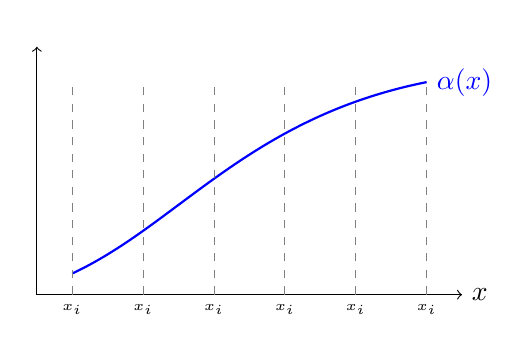
\begin{tikzpicture}[scale=0.9]
  \draw[->] (0,0) -- (6,0) node[right] {$x$};
  \draw[->] (0,0) -- (0,3.5) node[above] {};
  \draw[thick, blue] (0.5, 0.3) .. controls (2,1) and (3,2.5) .. (5.5, 3) node[right] {$\alpha(x)$};
  \foreach \x in {0.5, 1.5, 2.5, 3.5, 4.5, 5.5} {
    \draw[dashed, gray] (\x, 0) -- (\x, 3);
    \node[below] at (\x, 0) {\tiny $x_i$};
  }
\end{tikzpicture}
\end{center}
The weight $\alpha$ increases across the partition; the sum $\sum G(x_{i-1}) \Delta \alpha_i$ weights $G$ by the jumps of $\alpha$.

\end{document}
